\documentclass[a4paper]{report}
\usepackage[spanish]{babel}
\usepackage[utf8]{inputenc}
\usepackage{graphicx}
\usepackage[document]{ragged2e}
\usepackage{pdflscape}
\usepackage[table]{xcolor}
\usepackage{lscape}
\usepackage{listings}
\usepackage{xcolor}

\lstdefinestyle{mystyle}{
    basicstyle=\ttfamily\footnotesize,
    breakatwhitespace=false,         
    breaklines=true,                 
    captionpos=b,                    
    keepspaces=true,                 
    numbers=left,                    
    numbersep=5pt,                  
    showspaces=false,                
    showstringspaces=false,
    showtabs=false,                  
    tabsize=2
}
\lstset{style=mystyle}

\title{Programa 7 - Gramatica No Ambigua}
\author{Leon Tejeda 2CM5}
\date{Enero 2021}

\begin{document}
\maketitle
\begin{flushleft}
PLANTEAMIENTO DEL PROBLEMA:

Elaborar un programa para procesar la gramática ambigua:

B -> (RB | e
R -> ) | (RR

Adicionalmente, el programa debe de contar con las siguientes características:

1. La cadena puede ingresar por el usuario o automáticamente.
2. Mandar a un archivo y en pantalla la evaluación de la gramática imprimiendo el símbolo que está evaluando, indicando que producción se aplico y la cadena evaluada.
4. La longitud máxima será manejar cadenas de 1,000 caracteres.

DESARROLLO:

Se realizo un menu para que el usuario decida si quiere generar una cadena aleatorio o si desea ingresarla manualmente.

Ya una vez con la cadena bien definida se empezara derivando la lenttra B, sera una proceso de LL(1)

Una vez cumpliendo con una condicional, se asignara la produccion correspondiente y se añadira en otra cadena auxiliar

Tambien se pondran condicionales para determinar que simbolo se desea expandir

Se mostrara en pantalla el procedimiento de evaluacion, y de igual manera se guardara en una archivo de texto

\newpage

CODIGO:

\lstinputlisting[language=python]{Programa7_Gramatica No Ambigua.py}

\newpage

FUNCIONAMIENTO:

Menu del programa
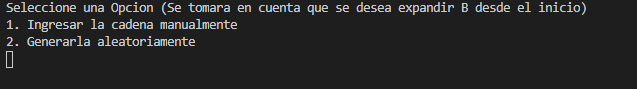
\includegraphics[width= 15cm, height= 5cm]{p7-1.png}

Cadena  = (())()- Modo Manual
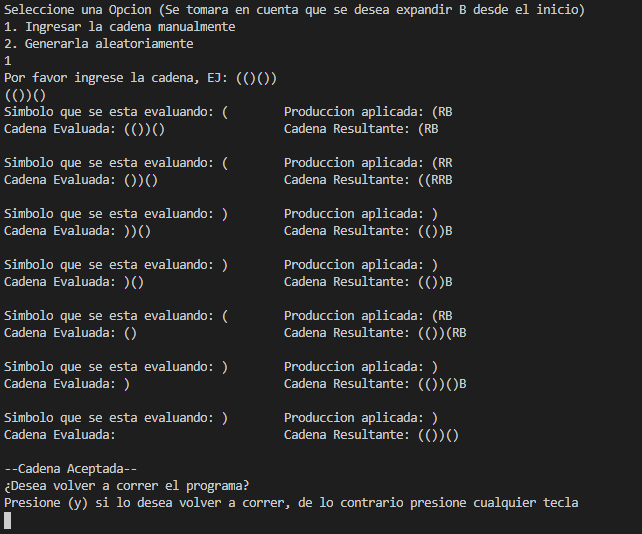
\includegraphics[width= 15cm, height= 5cm]{p7-2.png}

Cadena  = )(((())()())((  - Modo Aleatorio
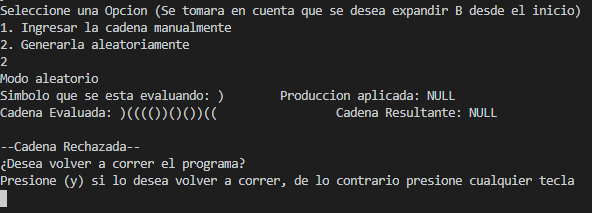
\includegraphics[width= 15cm, height= 5cm]{p7-3.png}

\end{flushleft}
\end{document}